\chapter{Graph Based Neuron Tracing} % Main chapter title

\label{T2T2_chapter} % For referencing the chapter elsewhere, use \ref{Chapter2} 

\lhead{Chapter 3. \emph{Tree2Tree-2}} % This is for the header on each page - perhaps a shortened title

In this chapter we will discuss our first neuron tracing algorithm, which uses graph theoretic algorithms to perform tracing. The proposed algorithm, Tree2Tree-2\cite{mukherjee_T2T_2} extends the former neuron tracer Tree2Tree, which was proposed by Basu \textit{et al.}\cite{basu_T2T_journal}. Both Tree2Tree and Tree2Tree-2 are hybrid algorithms in a sense that they combine strategies of both segmentation based techniques and graph based tracing. The idea is to start with an initial set of neurite segments, which are possibly disjoint, and then identify the connectivity between them. In the next few sections, we will discuss the properties of Tree2Tree-2 in more detail.

\section{Tree2Tree-2}
The general workflow of Tree2Tree-2  consists of three major steps: image denoising and filament enhancement, initial segmentatation and connectivity analysis .
\begin{figure}[t]
\centering
\begin{tabular}{c}
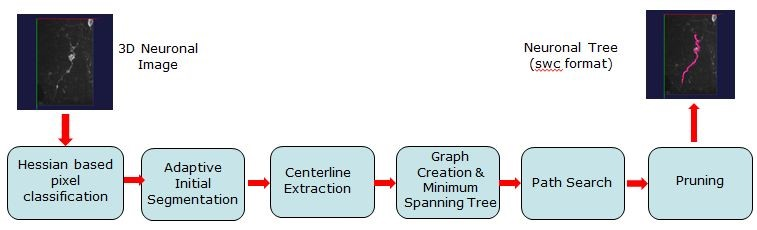
\includegraphics[width=0.8\linewidth]{./images/ch3/T2T2_pipeline.jpg}	
\end{tabular}
\caption[Tree2Tree-2: workflow]{The working pipeline of Tree2Tree-2}
\label{fig:T2T2_pipeline}
\end{figure}


\subsection{Hessian based vessel enhancement}
Frangi's \cite{frangi_vesselness} method for enhancing vascular structures is based on analyzing the geometric features of tubular objects. The vesselness or tubularity measure at a point $\textbf{x}\in \Omega$ in the image $f:\Omega \rightarrow \mathbb{R}$ can be obtained by examining the hessian matrix of the gaussian smoothed image over a set of scales. The hessian of the $d$-dimensional image $f(\textbf{x})$ at a position \textbf{x} and scale $\sigma$ is the square matrix $\mathcal{H}_{\sigma}(\textbf{x})=\left[ h \right]_{i,j} $ ($1\leq{i,j}\leq{d}, \; \textbf{x}\in\Omega$) which is given by
\bea
	 h_{i,j}=\frac{\partial^2G(\sigma)}{\partial x_i \partial x_j}*f(\textbf{x})
\eea 
Here \textbf{x} is the $d$-dimensional vector $\textbf{x}=\left(x_1,\ldots, x_d \right)^T$, $G(\sigma)$ is the zero mean normalized Gaussian kernel with variance $\sigma^2$. Here $d=2 $ or 3 for 2-D or 3-D images respectively.

At any position $\textbf{x}$ on the image surface, the local curvature in the direction of the vector $\textbf{v}$ is given by $\textbf{v}^T\mathcal{H}_\sigma(\textbf{x})\textbf{v}$. If $\textbf{v}$ is the direction along the vessel centerline (or major axis if we approximate a vessel locally as a cylinder), we expect the curvature to be negligible, assuming that the vessel intensity is homogeneous. On the other hand, in the directions orthogonal to the vessel axis, we encounter significantly higher curvature. Therefore, based on these curvature values, one can develop a discriminatory function (\textit{vesselness}) to differentiate between vascular and non vascular objects.

\subsubsection{Tubularity field}
From the above discussion, at a position $\textbf{x}\in \Omega$, a 3-D tubular structure can be characterized by three principal directions:
(i) an axial direction along which the second derivative is negligible, and (ii) two orthogonal directions along which the second derivative magnitude is significant. These directions are given by the orthonormal set of eigenvectors $\{\textbf{e}_1\left(\textbf{x}\right),\textbf{e}_2\left(\textbf{x}\right),\textbf{e}_3\left(\textbf{x}\right)\}$ of the hessian matrix(see Fig.~\ref{fig:frangi_vessel}(a)). The corresponding second derivative magnitudes or the curvature values are obtained from the respective eigenvalues as follows: $|\lambda_1(\textbf{x})|\leq{|\lambda_2(\textbf{x})|\leq{|\lambda_3(\textbf{x})|}}$.
\begin{figure}[t]
\centering
\begin{tabular}{ccc}
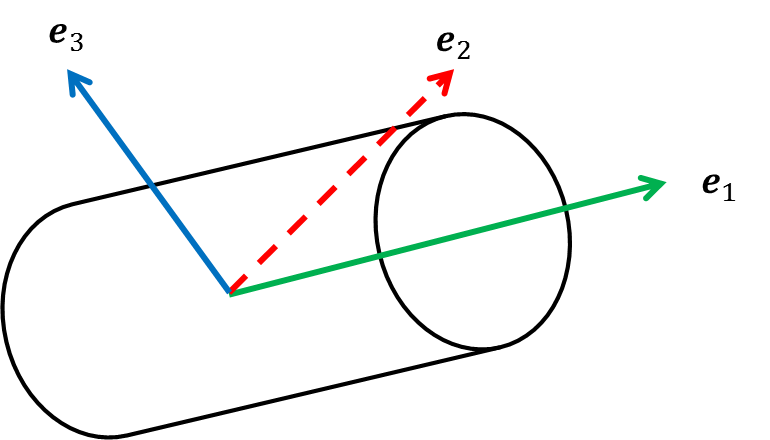
\includegraphics[width=0.3\textwidth]{images/ch2/3dvessel}	&
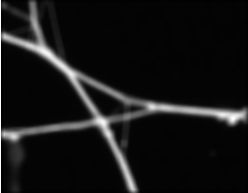
\includegraphics[width=0.25\textwidth]{images/ch2/vessel}	&
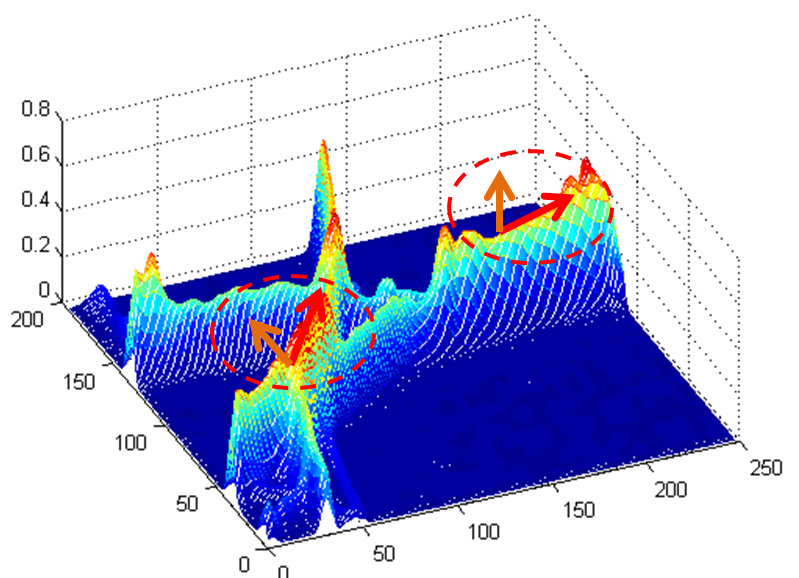
\includegraphics[width=0.3\textwidth]{images/ch2/vessel_mesh} \\
\scriptsize(a) & \scriptsize(b) & \scriptsize(c) \\
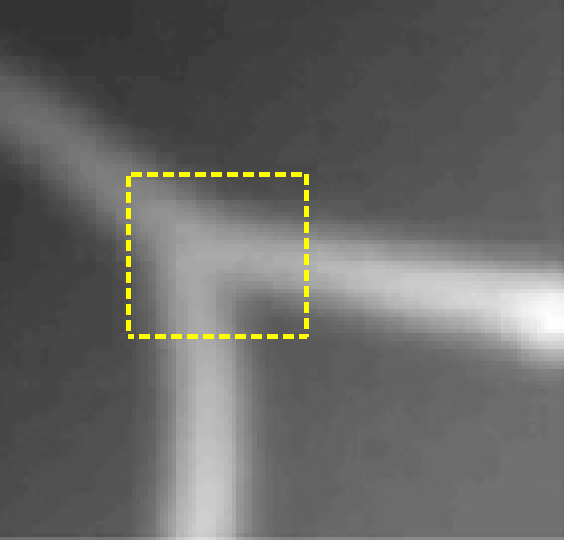
\includegraphics[width=0.28\textwidth]{images/ch2/orig}	&
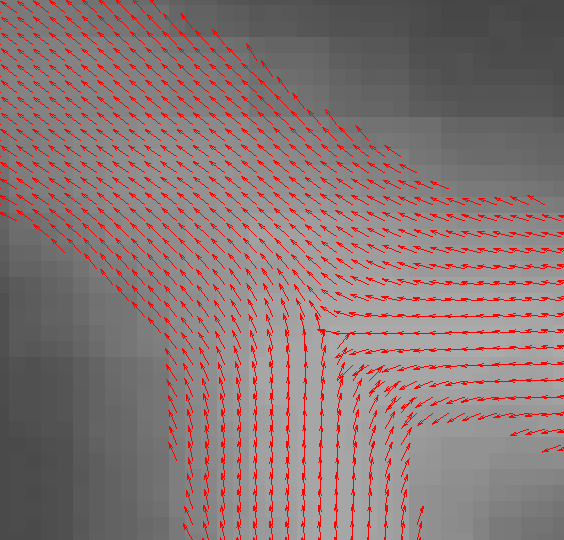
\includegraphics[width=0.28\textwidth]{images/ch2/F1}	&
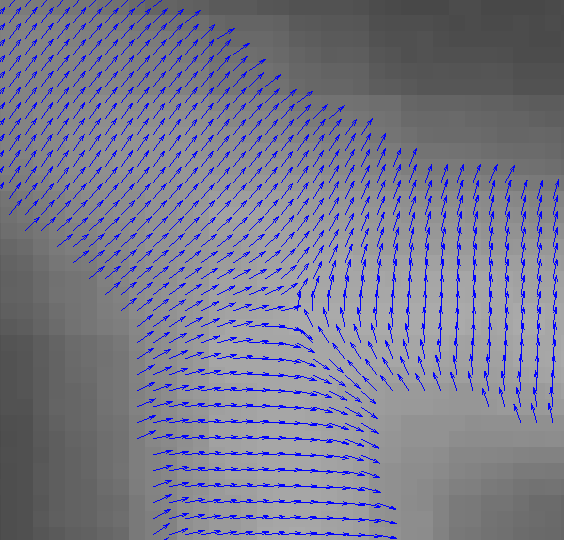
\includegraphics[width=0.28\textwidth]{images/ch2/F2} \\
\scriptsize(d) & \scriptsize(e) & \scriptsize(f) \\
\end{tabular}
\caption[Tubularity field]{(a) Graphic demonstration of the tubularity fields. (b) An image of a neurite and (c) corresponding surface plot of the image. Vessel orientations are shown by the red and orange vectors. This figure is best viewed in color. (d) A real example of a vascular structure. (e) Axial field $\textbf{e}_1$ and (f) Normal field $\textbf{e}_2$ for the zoomed portion.}
\label{fig:frangi_vessel}
\end{figure}
It may be observed that for a filamentous voxel \textbf{x}, the eigenvalues of its hessian matrix (computed at scale $\sigma$) should satisfy the following criteria:
\begin{gather}
\label{eq:3d_hessian}
|\lambda_1(\textbf{x})|\approx 0 \nn\\
|\lambda_2(\textbf{x})|\gg|\lambda_1(\textbf{x})|,\;|\lambda_3(\textbf{x})|\gg|\lambda_1(\textbf{x})| \\
|\lambda_2(\textbf{x})|\approx|\lambda_3(\textbf{x})|  \nn
\end{gather}
Also, assuming that vascular filaments are brighter than the background, we have  $\lambda_2(\textbf{x})<0$ and $\lambda_3(\textbf{x})<0$. A voxel that belongs to a vessel should satisfy the above mentioned criteria. Based on that, there has been several vessel enhancement measures proposed in the literature \cite{frangi_vesselness,basu_T2T_journal}.  For example, Basu \textit{et al}. \cite{basu_T2T_journal} suggests the following vesselness function $N_\sigma$ at scale $\sigma$  for enhancing the tubular structures:
\bea
	N_{\sigma}(\textbf{x})=
	\begin{cases}
		\dfrac{|\lambda_1(\textbf{x})-\lambda_2(\textbf{x})|^2}{|\lambda_1(\textbf{x})||\lambda_2(\textbf{x})-\lambda_3(\textbf{x})|} & \text{if $\lambda_2(\textbf{x}),\lambda_3(\textbf{x})< 0$} \\
		0 & \text{otherwise}
	\end{cases}
\eea
Also, since the filament thickness can vary, a multiscale analysis is essential. This can be evaluated by computing the maxima across a set of predefined scales, known as the scale space $S=\{\sigma_{min},\ldots,\sigma_{max}\}$.
\bea
	\sigma^*(\textbf{x})=\arg\!\max_{\sigma \in S}N_{\sigma}(\textbf{x}) \label{eq:optimal_scale}\\
	N(\textbf{x})=\max_{\sigma \in S}N_{\sigma}(\textbf{x}) \label{eq:vesselness_scale}
\eea
The scale space vesselness function $N(\textbf{x})$  assumes higher value at locations of local tubularity over non-filamentous positions. It should be noted that (\ref{eq:vesselness_scale}) yields evidence of the presence of vasculature by suppressing the non-filamentous structures, thus introducing a mechanism for dealing with noise and non tubular clutter.

\subsection{Initial Segmentation}

\begin{figure}[thb]
\centering
\begin{tabular}{ccc}
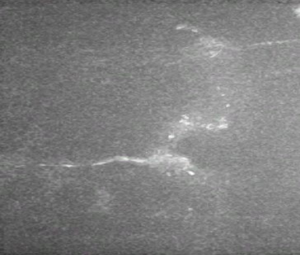
\includegraphics[width=0.3\linewidth, height = 0.25\linewidth]{./images/ch3/raw_demo}	&
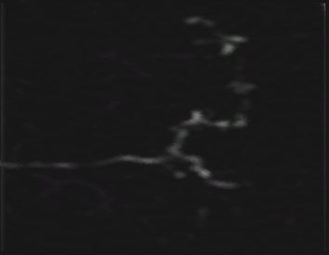
\includegraphics[width=0.3\linewidth, height = 0.25\linewidth]{./images/ch3/hessian_demo}	&
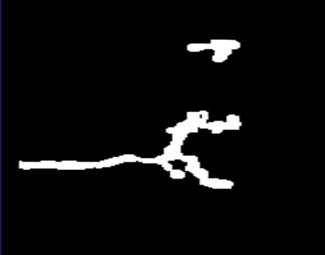
\includegraphics[width=0.3\linewidth, height = 0.25\linewidth]{./images/ch3/binary_demo}	\\
\scriptsize (a) & \scriptsize (b) & \scriptsize (c)
\end{tabular}
\caption[Tree2Tree-2: Initial segmentation]{Illustration of the enhancement and initial segmentation stage of Tree2Tree-2. (a) 3-D confocal image, (b) hessian enhanced image $N(\textbf{x})$ and (c) binary image, showing the two disjoint connected components after thresholding.}
\label{fig:T2T_enhance}
\end{figure}
Once the raw confocal image is denoised and the vessel contrast improved using the aforementioned technique, the obtained vesselness function (\ref{eq:vesselness_scale}) is segmented to get an initial estimate of neurite locations. The major aspect of Tree2Tree-2 is to integrate the possibly disjoint components obtained in the segmentation step. Since the connectivity analysis step is non-generative, we choose a local segmentation technique using variational minimax\cite{saha_minimax} to get a possibly overestimated solution having multiple binary connected components. The mathematical formulation of our segmentation framework is presented here.

Let $f:\Omega\mapsto\mathbb{R}$ be an image, and $N$ denotes the vesselness function which is computed using (\ref{eq:vesselness_scale}). We define a threshold surface $s(\textbf{x})$, $\textbf{x}\in\Omega$ such that our initial  segmentation result is given by the binary image $b:\Omega\mapsto \{0,1\} $ which is defined as follows:
\bea
	b(\textbf{x})=
	\begin{cases}
		1 & \text{if $N(\textbf{x})>s(\textbf{x})$} \\
		0 & \text{otherwise}
	\end{cases}
	\label{eq:minimax_binary}
\eea
The optimal threshold surface is computed by minimizing a convex energy functional $E(s,\alpha)$
\bea
E(s,\alpha) =\displaystyle \dfrac{1}{2}\sqrt{1-\alpha^2}\underbrace{\int_{\Omega}\left(N-s\right)^2|\nabla N|^2 d\textbf{x}}_{E_1} + \dfrac{1}{2}\alpha\underbrace{\int_{\Omega}|\nabla s|^2 d\textbf{x}}_{E_2}
\label{eq:minimax_func}
\eea
The first term in (\ref{eq:minimax_func}), $E_1$ is the data term, which computes the weighted mean square distance between the threshold function  the vesselness function. The second term, $E_2$ is a smoothness enforcing term that restricts the threshold function to develop high gradients. The relative contribution of these two functionals is controlled by the  parameter $\alpha$.

The gradient of the vesselness map corresponds to the filament edges. Therefore, the data term of the energy functional is significantly high at the filament edges, and the threshold function $s(\textbf{x})$ should be close to $N(\textbf{x})$ at edge position to reduce the cost functional in (\ref{eq:minimax_func}).

We seek to minimize (\ref{eq:minimax_func})  and since $E(s,\alpha)$ is convex with respect to $s(\textbf{x})$, the minimizing function $s^*$ is a global minima. Also, further analysis of (\ref{eq:minimax_func}) suggests that the functional is concave with respect to the scalar parameter $\alpha$. It may be observed that the characteristics of $E_1$ and $E_2$ are conflicting in a sense that the minimizer of $E_1$ does not entirely satisfy $E_2$, and vice-versa. One solution to this parameter selection problem is to use minimax technique. In a minimax paradigm, the optimal threshold surface is the one which minimizes the worst case cost function. Mathematically, this is stated as:
\bea
\{s^*(\textbf{x}),\alpha^*\} = \text{arg}\max_\alpha\min_s E(s(\textbf{x}),\alpha)
\label{eq:minimax_formulate}
\eea
We solve (\ref{eq:minimax_formulate}) using variational calculus for $s$, and the  obtained Euler-Lagrange equation is solved using gradient descent. We use alternating maximization to compute  $\alpha$. The solution is derived as follows. Please refer to the Appendix \ref{AppendixTuFF} for details of derivation.
\bea
\dfrac{\partial s}{\partial t} &=& \sqrt{1-(\alpha^*)^2}|\nabla N|^2\left(N-s\right)+\alpha^*\nabla^2 s\nn \\
\alpha^* &=&\dfrac{E_2}{\sqrt{E_1^2+E_2^2}}
\label{eq:minimax_soln}
\eea
We solve (\ref{eq:minimax_soln}) via discrete approximation of the partial differential equation, with Neumann boundary conditions. The optimal threshold  surface  is obtained at convergence, and then the initial segmentation $b(\textbf{x})$ is derived using (\ref{eq:minimax_binary}). The initial segmentation gives us an estimate of the neuron morphology. However, the imaged neurons may appear fragmented due to imaging artifacts. This can create multiple segments, instead of getting a single connected component (see Fig. ~\ref{fig:T2T_enhance}(c)), some of which may not belong to the original neuron. Therefore, to establish the global neural morphology, we introduce a method to analyze the connectivity between the different fragments, followed by a specialized pruning step to discard clutter.

\subsection{Connectivity analysis and component linking}
\begin{figure}[bht]
\centering
\begin{tabular}{cc}
\includegraphics[width=0.62\linewidth]{./images/graph_connectivity_a}	&
\includegraphics[width=0.3\linewidth]{./images/graph_connectivity_b}	\\
\scriptsize (a) & \scriptsize (b) 
\end{tabular}
\caption[T2T2: establishing global graph]{(a) The calculation of orientation and distance between leaf pairs. 2 synthetic connected components $C_i$ and $C_j$ shown in blue. 6 pairs of leaf node connectivity (shown in dotted green) are tested for the closest distance between the components. The closest leaf pair is indicated. (b)Two disjoint components are joined by the global connectivity algorithm (shown in red). However, the actual path is unknown and is decided by PathSearch.}
\label{fig:T2T2_conn}
\end{figure}
The primary contribution of Tree2Tree-2 is to analyze and determine proper connectivity between the disjoint segments (see Fig.~\ref{fig:T2T2_conn}). We adopt a graph theoretic approach to determine possible connections between the branches. Once this is established, the next step would be to physically link the components by a curve which traces the medial axis of the neurite filaments. 

The initial segmentation procedure classifies the image voxels into neuronal (foreground) and non-neuronal (background) portions, as shown in Fig.~\ref{fig:T2T_enhance}(c). Since the obtained foreground segments may be disjoint, the next step is to connect the components to obtain a global graph, and eventually, the neuronal tree. To ensure proper connectivity, we adopt a two stage procedure.

Let us denote the set of disjoint components as  $C=\{C_1,\ldots,C_n\}$.  The first step involves a global graph connectivity algorithm that decides  the connectivity between these components. The edge weights of the complete graph, created with the set of nodes $\{C\}$ are computed such that more probable connections have lower weights. Basu \textit{et al}.\cite{basu_T2T_journal} designed the edge weight function such that the weight $D_{ij}$ is low when two components $C_i$ and $C_j$ are close according to the euclidean distance metric and they are oriented towards each other. Mathematically, this is can be stated in the following manner: 
\bea
D_{ij} = \lambda \textit{dist}(C_i,C_j) + (1-\lambda)\textit{orientation}(C_i,C_j)
\label{eq:T2T2_globalgraph}
\eea
Here $dist()$ is a function that computes the shortest euclidean distance between the terminals of $C_i$ and $C_j$. The function $orientation()$ assumes a high value if the outward leaf tangent vectors of the connected components are facing in the same direction. An illustrative example is shown in Fig.~\ref{fig:T2T2_conn}(a). For detailed description, we refer the reader to the original paper \cite{basu_T2T_journal}.

A Minimum Spanning Tree (MST) of the global graph produces an initial neuronal tree. This method is computationally simple and provides efficient and accurate connectivity information between the components. The objective now is to detect the actual path that connects them in the image domain.

We devise a novel algorithm, PathSearch, which finds the  physical connection (in the image domain) between the components which are deemed suitable for joining in the initial graph based analysis step. 

\subsection{PathSearch}

The PathSearch algorithm to find the physical path between the terminal points of two disjoint components uses Dijkstra's method \cite{dijkstra1959note} to find the shortest path between the end points. Treating each voxel as a node in a graph, the edge weight between two neighboring voxels $\textbf{x}$ and $\textbf{y}$ is computed as
\bea
w(\textbf{x},\textbf{y})=\frac{2}{\mu(\textbf{x})+\mu(\textbf{y})}
\label{eq:pathsearch}
\eea
Non-neighbors are not connected by an edge. Here, we assume 26-connectivity of the voxels in 3D (8-connectivity in 2D). $\mu(\textbf{x}),\mu(\textbf{y})$ denote the medialness value at voxel positions $\textbf{x}$ and $\textbf{y}$, which assumes a higher value at voxels near the medial axis than those away from the medial axis\cite{mukherjee_medialness}\footnote{For implementation, only a subset of pixels in a window containing the two endpoints are considered, to make processing faster.}. Choice of this weight function ensures that two voxels on a neuron medial axis are connected by a lower edge weight than two arbitrary, non-neuronal voxels. With this edge weight defined on the graph, we now use Dijkstra's shortest path algorithm \cite{dijkstra1959note} to determine the path connecting the end points between two segments. To get a smooth connection, we further interpolate this path by fitting a cubic B-spline to this curve. The workflow of the PathSearch method can be summarized as follows:
\begin{enumerate}
\item Determine the  connectivity between the end nodes of the disjoint binary components using relative orientation and euclidean distance between the components.
\item Compute the neuron tree using MST.
\item Compute a medialness map to produce evidence of a path along neuron medial axis (cf. \cite{mukherjee_medialness}).
\item Join the end points (in the image domain) by computing the shortest path between them using suitable edge weight function.
\item Smooth the obtained trace by spline fitting.
\end{enumerate}

\section{Multiscale medialness map}

In the previous section, we mentioned that the PathSearch algorithm joins the components via shortest path along the medial axis of the underlying neuron. This requires computing a \textit{medialness} function $\mu(\textbf{x})$ (see (\ref{eq:pathsearch})), which assumes higher values at the object medial axis. 

Finding medial axis for binary structures is a well studied problem in mathematical morphology\cite{bovik2010handbook}. However, the problem is non trivial for gray scale objects. In this section, we introduce a technique for computing a medialness map for non binary objects and we use the computed medialness value for neuron tracing via Tree2Tree-2. 

\subsection{Vector field convolution medialness}
\begin{figure}[thb]
\centering
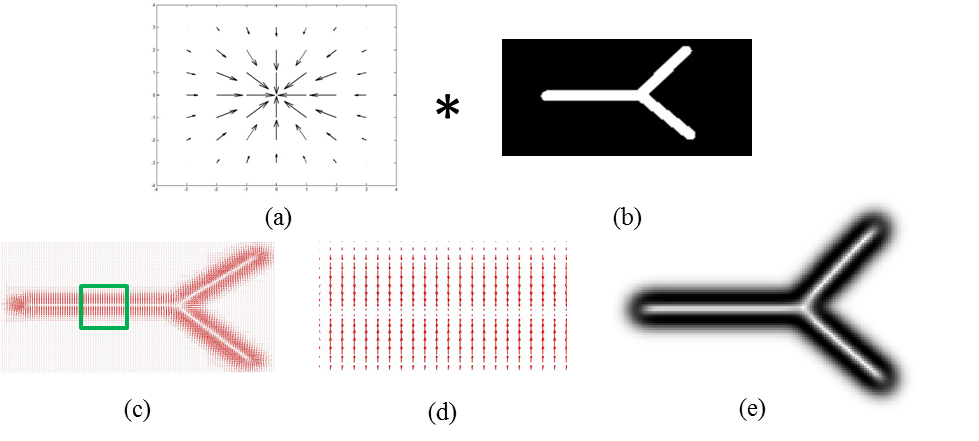
\includegraphics[width=1\linewidth]{./images/VFC/medialness}	
\caption[VFC medialness]{A discrete VFC kernel is shown in (a). (b) shows a synthetic tubular structure. (c) illustrates the vector fields after convolving (b) with the kernel, at some scale. An enhanced view is shown in (d), which reveals that the vectors cancel at the medial axis. The computed scale-space medialness map is shown in (c).}
\label{fig:medialness}
\end{figure}
\noindent We propose a novel method to compute the medialness function of a grayscale object using vector field convolution (VFC) [11], which is computationally efficient and robust to noise. The vector field convolution kernel is defined as
\bea
K_{\gamma}(\textbf{x})=m_\gamma(\textbf{x})\frac{\textbf{x}}{||\textbf{x}||}
\label{eq:VFC_ker}
\eea
The kernel is designed such the the vectors are directed towards the kernel center $\textbf{x}=0$. Magnitude of the vectors is determined by the magnitude function $m_\gamma(\textbf{x})$. Choosing $m_\gamma(\textbf{p})=\exp(-||\textbf{p}||^{2}/\gamma^{2})$, we create a kernel such that the influence of the vector field diminishes away from the center. This \emph{kernel range} can be tuned by the scale parameter $\gamma$. A sample VFC kernel is shown for illustration in Fig.~\ref{fig:medialness}(a). At the correct scale, convolution of an image with the VFC kernel produces a zero magnitude vector at the points of symmetry of the grayscale object, since the vectors cancel each other. The points of symmetry of an object can be recognized by finding the local minima in the convolved image (assuming the object is brighter than the background). Mathematically, at a scale $\gamma$, the vector field obtained after convolving the image $f(\textbf{x})$ with the kernel in (\ref{eq:VFC_ker}) is given as $V_{\gamma}(\textbf{x})= f(\textbf{x})*K_{\gamma}(\textbf{x})$. At this particular scale, the medialness is defined as
\bea
\mu_{\gamma}(\textbf{x})=1-\frac{|V_{\gamma}(\textbf{x})|-\min|V_{\gamma}|}{\max|V_{\gamma}|-\min|V_{\gamma}|}
\label{eq:med_scale}
\eea

\subsection{Multiscale VFC medialness}
Since the neurite thickness varies, a multiscale approach is required to obtain a scale invariant medialness function.  Let $\Theta$ be the scale space, which captures thickness of the objects of interest. In order to evaluate the correct medialness response over the scale space, we observe that the medialness response of a non-medial point diminishes with increasing scale, whereas, the response is significant for the medial points for each scale. The scale space medialness map is computed as
\bea
\mu(\textbf{x})=\frac{1}{|\Theta|}\sum_{\gamma \in \Theta}\mu_{\gamma}(\textbf{x})
\label{eq:medialness_map}
\eea
Fig.~\ref{fig:medialness} illustrates the medial map computation on a synthetic tubular object. Fig.~\ref{fig:medialness}(c) shows the vector field, which is generated by convolving the image (b) with the VFC kernel (at a fixed scale). The scale space medialness map is shown in Fig.~\ref{fig:medialness}(e). 


\section{Computing the neuronal tree}
To summarize Tree2Tree-2, we first compute a global neuron tree using MST, where the connectivity information between the terminals of the neurite fragments are derived based on the relative geometry of the components. Then, PathSearch is used to physically connect the endpoints, by finding the shortest path between the terminals, which adheres to the medial axis of the neurite filaments.
Let us designate the global tree obtained using MST and PathSearch as $\Gamma=\{E,V,W\}$. Here $E = \{e\},V=\{v_{ij}\}$ and $W=\{w_{ij}\}$ denote the sets of edges, nodes and edge weights of the global tree.
The  nodes $v\in V$ correspond to the individual segments obtained after initial segmentation, and the edges $e_{ij}\in E$ between the nodes $(v_i,v_j)$  are computed via PathSearch. To assign the weight $w(e_{ij})\in W$ to an edge $e_{ij}$, we compute the sum of the edge weights of the shortest path between $v_i$ and $v_j$. This ensures that false edges have a higher path weight than the true connections. 

However, since the initial segmentation step may result in over segmentation, we may eventually get undesired nodes in the neuron tree due to the presence of clutter. 
This leads to the final step of Tree2Tree-2, where a pruning methodology is deployed to eliminate the false nodes.
\subsection{Tree pruning}
\begin{figure}[t]
\centering
\begin{tabular}{cc}
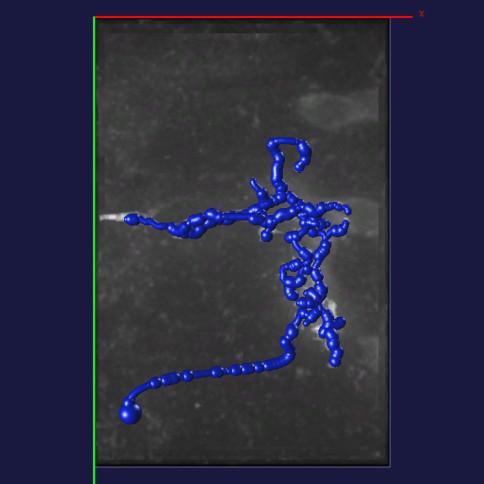
\includegraphics[width=0.4\textwidth]{images/ch3/clutter1}	&
\includegraphics[width=0.4\textwidth]{images/ch3/clutter1_pruned}	\\
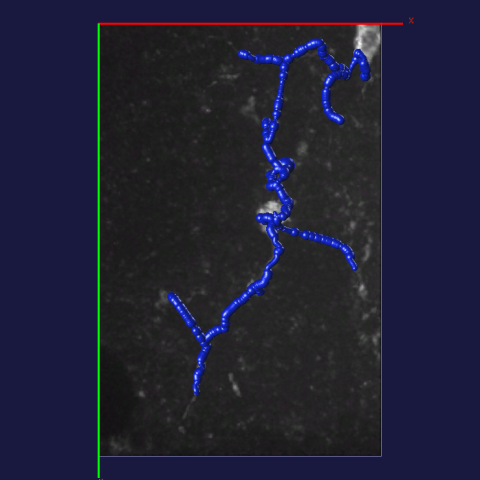
\includegraphics[width=0.4\textwidth]{images/ch3/clutter2}	&
\includegraphics[width=0.4\textwidth]{images/ch3/clutter2_pruned}	\\
\scriptsize(a) & \scriptsize(b)
\end{tabular}
\caption[Tree2Tree-2 graph pruning]{Results of graph pruning. (a) A global neuron tree using MST+PathSearch. (b) The pruned tree with the false nodes removed.}
\label{fig:T2T2_pruning}
\end{figure}
We designate the volume (area) occupied by a tree in the 3D (2D) binary image as $\psi(\Gamma)$. Our assumption is that the neuronal portions occupy more volume than the clutter, and the cost of connecting them via PathSearch is more compared to a true node. We devise the following method to prune the tree: 

Let $e\in E$ be an edge in the tree, i.e.$w(e)\geq w(e'),\, \forall e\in E$. Removing this edge from the tree $\Gamma$ creates two disjoint subtrees $\Gamma_1$ and $\Gamma_2$. Let us denote $\Gamma^* = \underset{\Gamma_j}{\arg\min}\,\psi(\Gamma_j)$. From standard graph theory, the graph $\Gamma\setminus\Gamma^*$ that results from removing the subtree $\Gamma^*$ from the global tree $\Gamma$, is also a subtree. 

Our strategy for pruning the tree is as follows. We select a scalar variable $\rho \in \left[0,1\right]$, which may be defined by the user.  The subtree $\Gamma^*$ is removed from the tree if $\dfrac{\psi(\Gamma^*)}{\psi(\Gamma)}\leq \rho$. The pruning process is repeated till no subtree can be further removed from the tree. Using this strategy, a subtree is deleted if it is connected by a significantly high cost path (which signifies higher possibility of a false connection), and the volume occupied by the subtree is small enough compared to the overall volume (since the area/volume of the clutter is significantly lower than the neurites). Typically, we use a low value of $\rho$$ (\approx 0.1)$, which  encourages removal of clutter over a neuron segment (Fig.~\ref{fig:T2T2_pruning}).
\begin{figure}[tb]
\centering
\begin{tabular}{cc}
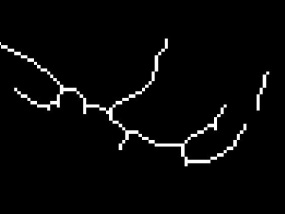
\includegraphics[width=0.4\textwidth]{images/ch3/broken}	&
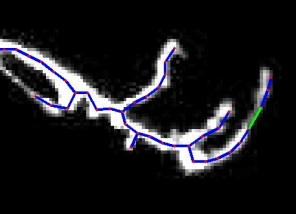
\includegraphics[height=0.302\textwidth]{images/ch3/connected}	\\
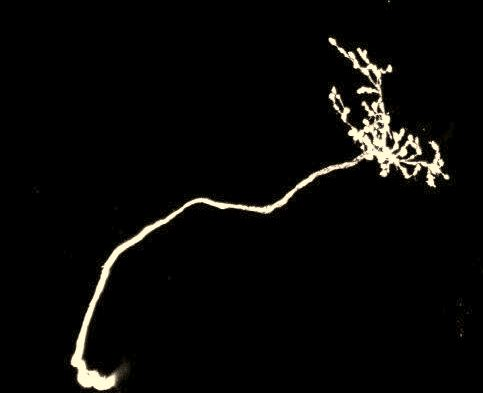
\includegraphics[width=0.4\textwidth]{images/ch3/n4}	&
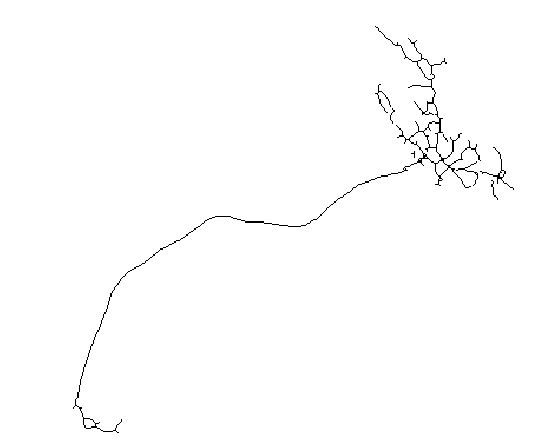
\includegraphics[width=0.4\textwidth]{images/ch3/n4_VFC}	\\
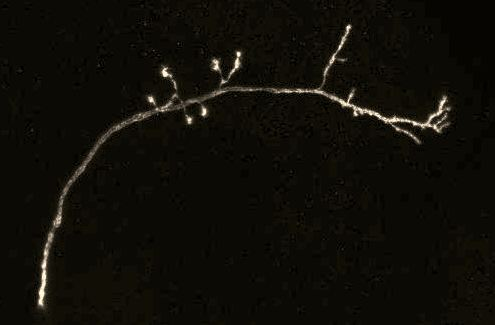
\includegraphics[width=0.4\textwidth]{images/ch3/n7}	&
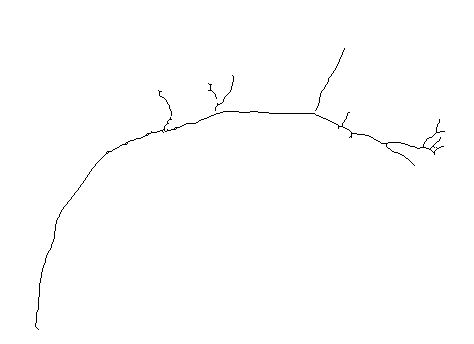
\includegraphics[width=0.4\textwidth]{images/ch3/n7_VFC}	
\end{tabular}
\caption[Tree2Tree-2: 2D results]{The top row shows an example how a broken link is joined by Tree2Tree-2 in 2D. The resulting tracing is shown in the second column and the detected connectivity is shown in green. Rows 2 and 3 show Tree2Tree-2 tracing results on 2D maximum intensity projection neuron images. The traced results are shown in the second column.}
\label{fig:T2T2_results2D}
\end{figure}

\section{Results}
Tree2Tree-2 is a tracing algorithm, applicable to both 2D and 3D images. We first present a few qualitative tracing results on 2D images. The 2D images are obtained using maximum intensity projection of the 3D stacks along the Z-axis (depth). Fig.~\ref{fig:T2T2_results2D} shows the tracing results of Tree2Tree-2 on a few 2D images. 
\begin{figure}[t]
\centering
\begin{tabular}{cc}
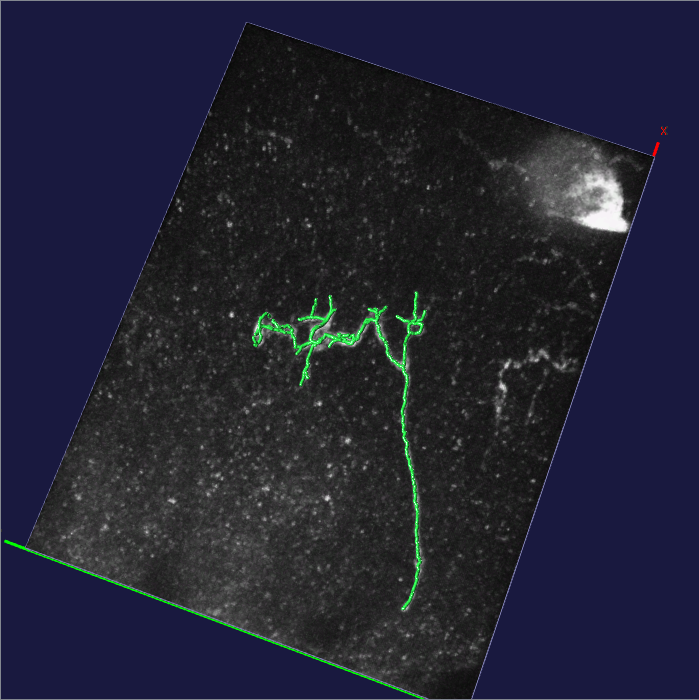
\includegraphics[width=0.4\textwidth]{images/ch3/T2T2_3D1_org}	&
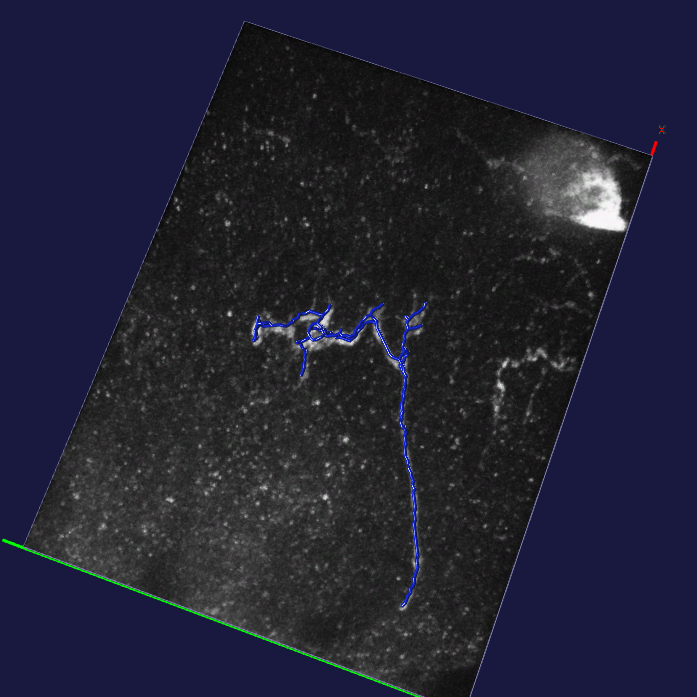
\includegraphics[height=0.4\textwidth]{images/ch3/T2T2_3D1}	\\
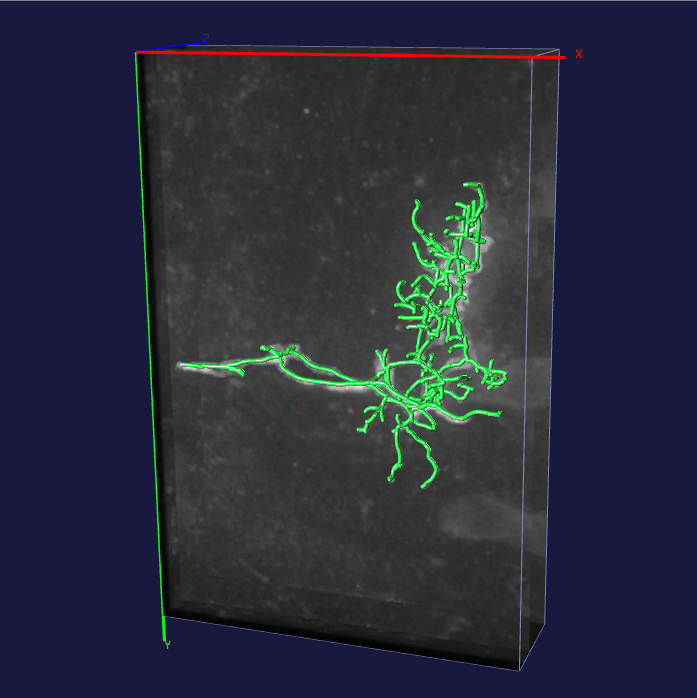
\includegraphics[width=0.4\textwidth]{images/ch3/T2T2_3D2_org}	&
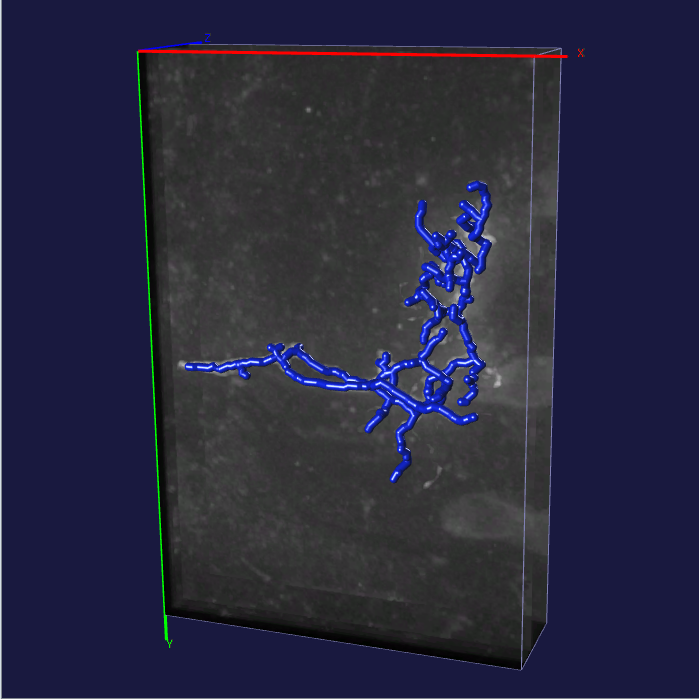
\includegraphics[width=0.4\textwidth]{images/ch3/T2T2_3D2}	\\
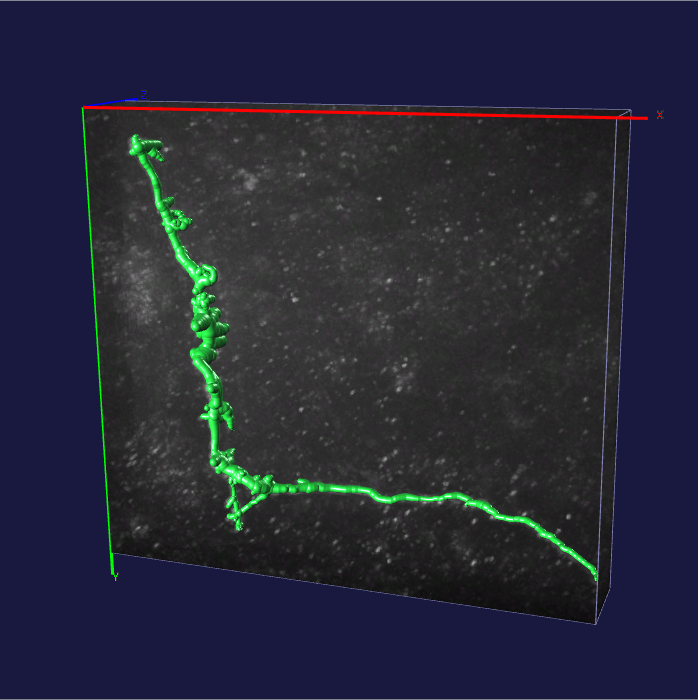
\includegraphics[width=0.4\textwidth]{images/ch3/T2T2_3D3_orig}	&
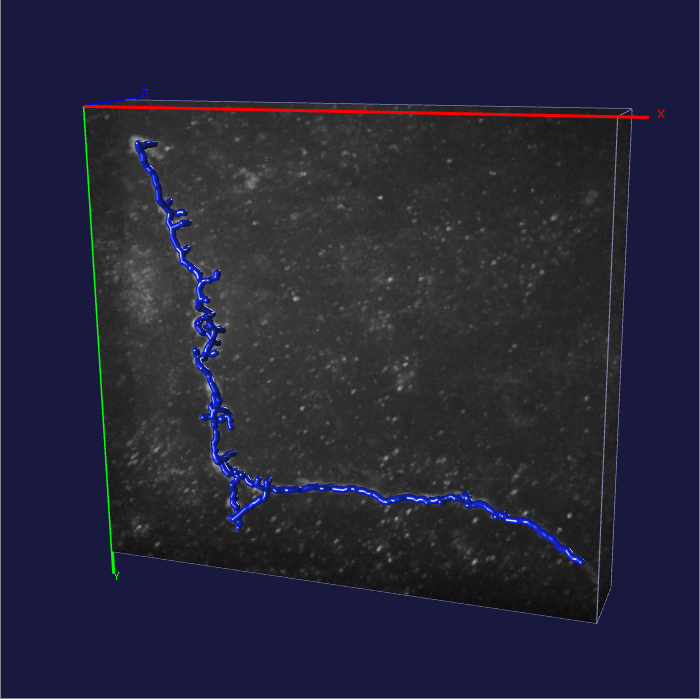
\includegraphics[width=0.4\textwidth]{images/ch3/T2T2_3D3}	
\end{tabular}
\caption[Tree2Tree-2: 3D results]{The first column shows manual tracing results(green). 3D tracing results of Tree2Tree-2 are shown in the second column (blue). The splined centerline is plotted on the original 3D confocal images of the Drosophila larva.}
\label{fig:T2T2_results3D}
\end{figure}
Qualitative results for 3D tracing are shown in Fig.~\ref{fig:T2T2_results3D}. The manual tracing results are shown in the first column, and are overlaid on the original images using the Vaa3D visualization software\cite{peng_v3d}. Tracing results due to Tree2Tree-2 are shown in the second column in blue. 

To quantify the performance of Tree2Tree-2, we use the normalized Mean Absolute Error (NMAE)\cite{basu_T2T_journal} of the traced neuron, with respect to the manually annotated tracings. Preliminary experiments were performed on a batch of ten 3D stacks, which contained noisy images of Drosophila neurites. We observed an average NMAE of 1.01\%, as compared to 1.97\% for that of its precursor algorithm Tree2Tree \cite{basu_T2T_journal}. The improvement in performance is largely due to the fact that Tree2Tree-2 uses PathSearch to compute the physical path between two objects, where Tree2Tree uses splines to interpolate the positions between two fragments. Also, the proposed tree pruning method in Tree2Tree-2 is simpler and more efficient compared to the alpha-beta pruning step in Tree2Tree.
\clearpage
\section{Discussion}
The proposed algorithm, Tree2Tree-2 is essentially a neuron tracing method which leverages the capabilities of graph theoretic algorithms to identify the centerlines of the neuron filaments. The primary contribution of Tree2Tree-2 is to determine the connectivity between the different binary objects, which are obtained via initial segmentation of the neurites. From that perspective, Tree2Tree-2 can be considered an intelligent component analysis algorithm. Using simple graph based methods, we are  able to compute the centerlines of neurites with considerable accuracy, given that the structural complexity is not significant. The initial segmentation step requires few parameters, and therefore helps automating the process. Moreover, Tree2Tree-2 revisits the component connectivity issue from the image domain perspective as well, once the initial connectivity information is obtained using graphs. This allows us to accurately connect the neurites along physical paths, as opposed to interpolating them in Tree2Tree. Also, since efficient algorithms exist to compute  MST and shortest paths, Tree2Tree-2 is computationally efficient.

However, on the downside, Tree2Tree-2 relies on the initial segmentation step. If components are lost during thresholding, the algorithm is unable to interpolate the neurite structure. Therefore, it is preferable that the initial segmentation overestimates the solution. 

However, such under segmentation can result in multiple binary components, which reduces the efficacy of the graph based connectivity analysis portion of Tree2Tree-2. In fact, since the neurite connections are analyzed only between the end points of the objects, it does not accommodate all possible cases of discontinuities. As a result, structural complexity of the filaments, as well as the number of binary objects in the solution degrades the tracing performance by predicting false edges between the fragments. Two examples are shown in Fig.~\ref{fig:T2T2_error}. In Fig.~\ref{fig:T2T2_error}(a), we demonstrate a 2D example, where the initial segmentation resulted in the tracing in blue. The green lines show the links predicted by Tree2Tree-2. The region highlighted by the red circle shows a situation, where the component connectivity cannot be resolved by analyzing the end points of the fragments. However, since Tree2Tree-2 cannot handle discontinuities which are not between the object termini, a false branch is predicted. A similar result is shown in (b) for a 3D image, where Tree2Tree-2 forces the objects to be connected between the two terminals. 
\begin{figure}[th]
\centering
\begin{tabular}{cc}
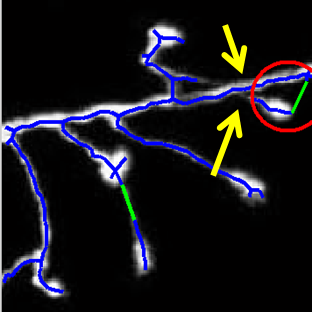
\includegraphics[width=0.45\textwidth]{images/ch3/error1}	&
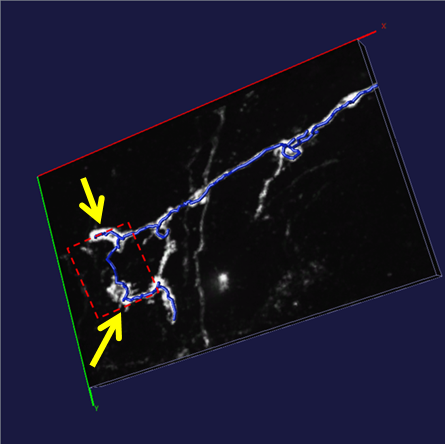
\includegraphics[height=0.45\textwidth]{images/ch3/error2} \\
\scriptsize (a) & \scriptsize (b)
\end{tabular}
\caption[Tree2Tree-2: connectivity errors]{Examples of false edge prediction by Tree2Tree-2. In both examples, error in connectivity results from Tree2Tree-2's inability to handle discontinuities which are not between the end points of the objects. Improper branch connections are highlighted  by yellow arrows. Regions enclosed by the red curves show the regions of interests. }
\label{fig:T2T2_error}
\end{figure}
While such a branch can be removed by pruning the tree, it would result in the removal of a subtree, which  contains a real neurite portion. Therefore, investing in  a pruning strategy is not the most effective way to solve this problem. We hypothesize that such connectivity related issues can be better handled if the segmentation methodology is naturally able to adapt to the object topology. For example, so far we have been interested in determining the appropriate connections between the objects; however, a segmentation method which does not require such explicit connectivity analysis would fare better in circumstances where the neuron structures are complicated. This motivates us to use geometric deformable models \cite{osher_sethian,caselles_geodesic} for segmenting complicated structures like neurons. In such a paradigm the object topology is handled automatically, and if the model is appropriately designed, there is no need to assess the connectivity information based on geometrical position of the objects. In the next chapter, we present a  brief overview of geometric active contours and surfaces for segmentation, and we formalize a procedure to use them for our application in the following chapters.
























